\documentclass{article}
\usepackage{times}
\usepackage{balance}
\usepackage{amssymb}
\usepackage{amsfonts}
\usepackage{amsmath}
\usepackage[amsmath,thmmarks]{ntheorem}
\usepackage{mathrsfs}
\usepackage[utf8]{inputenc}
\usepackage{listings}              % code insert
\usepackage{graphicx}
\usepackage{rotating}

\newcommand{\R}{\mathbb{R}}
\newcommand{\C}{\mathbb{C}}
\newcommand{\Z}{\mathbb{Z}}
\newcommand{\id}{\textrm{id}}
\newcommand{\pr}{\mathrm{pr}}
\newcommand{\N}{\mathbb{N}}


\newtheorem{thm}[equation]{Theorem}
\newtheorem{lem}[equation]{Lemma}
\newtheorem{prop}[equation]{Proposition}
\newtheorem{cor}[equation]{Corollary}
\newtheorem{conj}[equation]{Conjecture}

\theoremstyle{plain}
\theorembodyfont{\normalfont}
\newtheorem{defn}[equation]{Definition}
\newtheorem{ex}[equation]{Example}
\newtheorem{claim}[equation]{Claim}

\theoremstyle{nonumberplain}
\theoremheaderfont{\normalfont\bfseries}
\theorembodyfont{\normalfont}
\theoremsymbol{\ensuremath{\square}}
\theoremseparator{.}
\newtheorem{proof}{Proof}


\pagestyle{plain}

\begin{document}

\title{Advanced Computer Systems \\ Assignment 4}

\author{Anna Sofie Kiehn and Kenneth Jürgensen}

\maketitle

\section*{Question 1: Recovery Concepts}

\subsection*{1}
	Since force is implemented there is no need for undo as all changes are written when comitted. Since there is no-steal no data is written before it is comitted, and therefore no undo scheme needs to be implemented as there can be no data that is written but not comitted.

\subsection*{2}
	Nonvolatile storage is storage that does not lose data when power is lost, like a harddisk. Stable storage is storage that which in theory can survive any kind of failure. Nonvolatile storage,while it does not lose data on power failure it is still succeptible to data corruption due to partially written data, where as stable storage can use replication of data to rule out corruption. However this replication of data also makes stable storage more computationally expensive than nonvolatile storage.

\subsection*{3}
	When the change to the database is to be written to disk, the write-ahead-log must be written to stable storage before the change is written. This is to ensure that no change of the state of the database can happen without being recorded for potential redo/undo in case of a crash.

\section*{Question 2: ARIES}

\subsection*{1}

Below is the state of the transaction and dirty page tables after the analysis phase.
The U in the transaction table, referes to the transactions needs to be undone.\\
\begin{tabular}{| c | c | c |}
	\hline
	\multicolumn{3}{|c|}{Transaction table} \\
	\hline
	transID & lastLSN & Status\\
	\hline
	T1 & 4 & U\\
	\hline
	T2 & 9 & U\\
	\hline
\end{tabular}
\begin{tabular}{| c | c |}
	\hline
	\multicolumn{2}{|c|}{Dirty page table} \\
	\hline
	pageID & recLSN \\
	\hline
	P2 & 3 \\
	\hline
	P1 & 4 \\
	\hline
	P5 & 5 \\
	\hline
	P3 & 6 \\
	\hline
\end{tabular}

\subsection*{2}

As we can see in the transaction table above the set of winner transactions are \{T3\}, as this T3 finishes before the crash, the set of losers are \{T1,T2\}, as they are both active when the crash happens.


\subsection*{3}
Redo phase starts at LSN 3 as that is the smallest recLSN in the dirty page table.\\
Undo phase ends at LSN 3 as that is the oldest log record of the transactions active at the crash and runs backwards through the log, starting from the tail.

\subsection*{4}
The set of log records that may cause page redos are \{3,4,5,6,8,9\}.

\subsection*{5}
The set of records that are undone is \{9,8,5,4,3\}. The undo phase starts at LSN 9 and undos all updates done by the looser transactions. 

\subsection*{6}
\begin{tabular}{ l  l  l  l  l  l }
	LSN & LAST\_LSN & TRAN\_ID & TYPE & PAGE\_ID & undoNextLSN \\
	- - - & - - - - - - - - & - - - - - - - & - - - - & - - - - - - - & - - - - - - - - - - - \\
	1 & - & - & begin CKPT & - & - \\
	2 & - & - & end CKPT & - & - \\
	3 & NULL & T1 & update & P2 & - \\
	4 & 3 & T1 & update & P1 & - \\
	5 & NULL & T2 & update & P5 & - \\
	6 & NULL & T3 & update & P3 & - \\
	7 & 6 & T3 & commit & - & - \\
	8 & 5 & T2 & update & P5 & - \\
	9 & 8 & T2 & update & P3 & - \\
	10 & 6 & T3 & end & - & - \\
	11 & - & T2 & CLR & P3 & 8 \\
	12 & - & T2 & CLR & P5 & 5 \\
	13 & - & T2 & CLR & P5 & NULL \\
	14 & - & T1 & CLR & P1 & 3 \\
	15 & - & T1 & CLR & P2 & NULL \\
\end{tabular}
We were a little unclear about if the records that are undone are removed from the log or if they are kept there, but the CLR record indicates that the record has been rolled back. We think that a log should never delete a record, once something has been logged that information should not be lost, so we show the log with the CLR to indicate that the records have been undone.

\section{Programming task}
\subsection{Setup for experiments}

\textbf{Generation of data:}
We implemented the random generation of books by rolling a random number between 0 and 1 billion as the isbn, to make it very unlikely that two threads wil generate two different books with the same isbn. The number of copies for each book is a random number between 1000 and 2000, the price is a random number between 100 and 600 and the title and author are random 10 character strings consisting of lower case letters and space. Every generated book has 0 in saleMisses, timesRated and totalRating and a random boolean in editorPick. The bookstore is always initiated with 20 books generated this way.\\\\
\textbf{Hardware:}
We ran the tests on a macbook with the following specs:
\begin{itemize}
	\item OS: OS X Yosemite version 10.10.5
	\item RAM: 8 Gb 1600 MHz DDR3
	\item CPU: 2 GHz Intel Core i7
\end{itemize}
\textbf{Workload configuration:}
We configured every worker to get up to 10 editorpicks and chose 5 books from this set to by 1 copy of each book as the client interaction which is run roughly 60\% of the total runs. For the replenishment interaction we chose to add 10 copies to the 5 books with the least copies, which is run about 30\% of the total runs. Finally for the stock acquisition interaction we chose to add 5 new books which is run roughly 10\% of the total runs.\\
For the local tests 100 warm up runs are used and 1000 actual runs are used, and for the RPC tests 10 warm up runs and 100 actual runs are used. This is because the overhead of RPC adds considerable latency, as can be seen in the plots later, which would take hours or more to run, but the workload for each run is the same for either test.\\
In the reporting of the metrics, we add up the total number of interactions, the total number of client interactions, the throughput and latency of each worker. All this information is used to validate that the number of client interactions constitute roughly 60% of the total interactions, that more than 99% of the interactions are successful and report the total throughput for all workers and the combined average latency as milliseconds between each interaction.


\subsection{Plots of throughput and latency}

\textbf{Throughput:}
Figure 1 shows the throughput at various amounts of concurrent clients when running the test locally and using RPC. Since the number for the local measurements are so much greater than the RPC ones it is hard to see the trends for RPC but they are roughly the same as for the local measurements except smoother due to the overhead RPC adds. From this plot it looks as if the throughput initially increases as the number of clients increases, but at a certain point the number of clients starts to reduce the overall throughput. This is to be expected as initially there will be a gain in throughput as one client will be able to utilize the wasted throughput that could be achieved when another client is not accessing the bookstore. However as more clients are added the potential wasted time from waiting for the bookstore to become available starts to hurt the overall throughput. 
The plot also shows an outlier in the data for the local measurement at 45 clients. Such outliers can be explained by the machine running the test running other applications in the background that might take up or free resources at various points. Had we run the measurement with an increment at intervals of 1 client instead of 5 the curve would probably have become much smoother and such outliers would stand out less but the time needed to run the measurement would also become much greater.\\
\textbf{latency}
 Figure 2 shows the latency at various amounts of concurrent clients when running the test locally and using RPC.

{\centering
\begin{figure}
	\hspace*{-2.2in}
	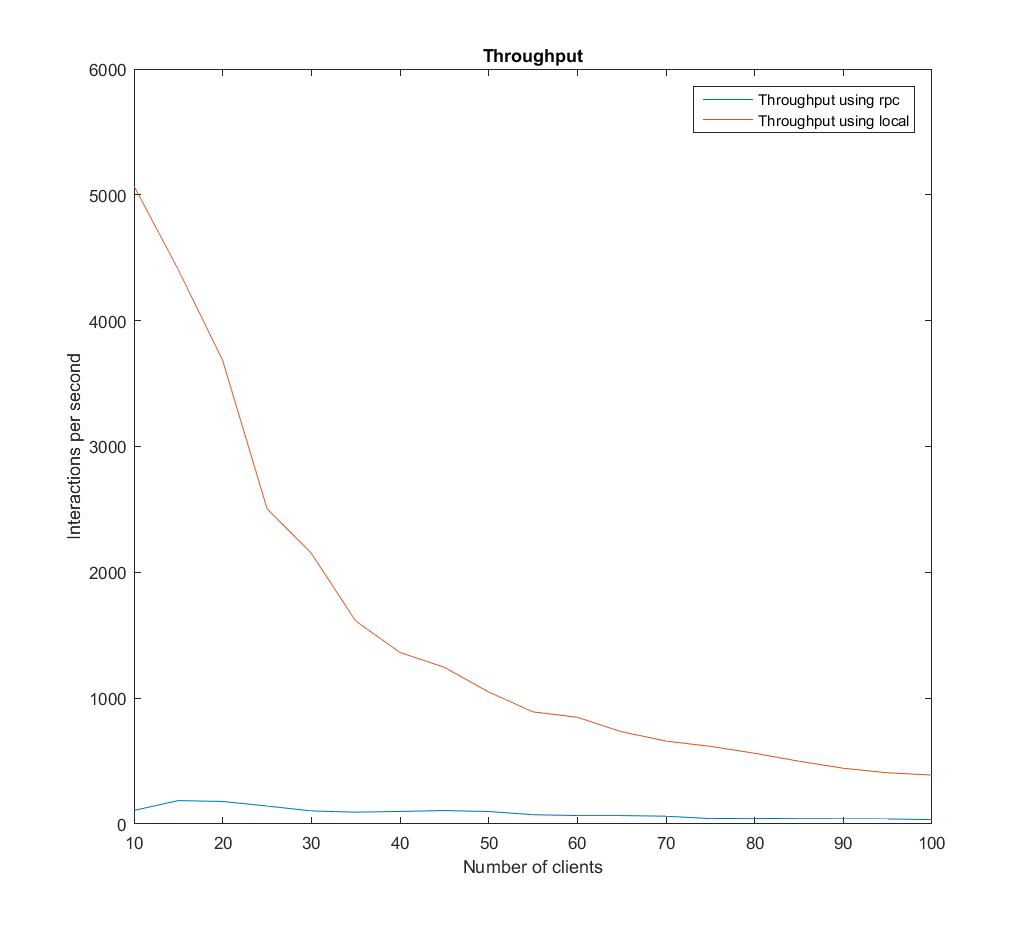
\includegraphics[scale=0.9]{throughput}
	\caption{Plot of the measurements of throughput}
\end{figure}
\begin{figure}
	\hspace*{-2.2in}
	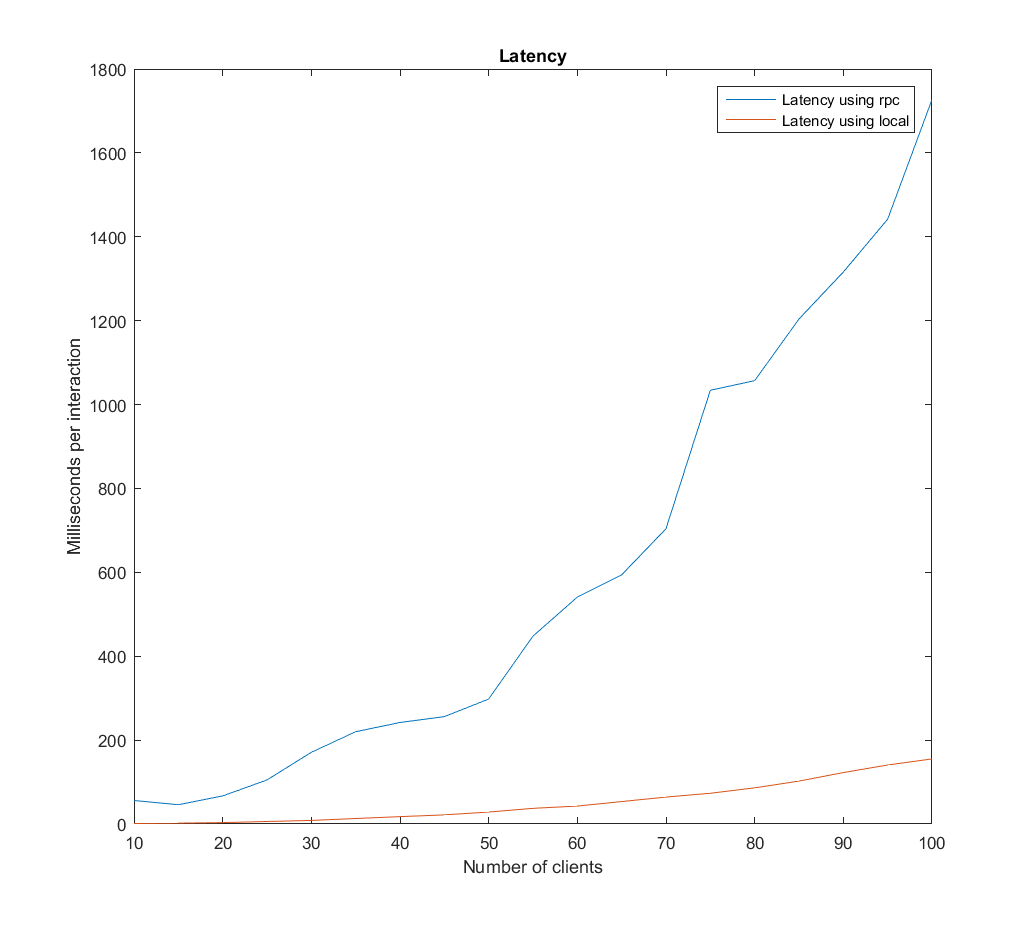
\includegraphics[scale=0.9]{latency}
	\caption{Plot of the measurements of latency}
\end{figure}}

\subsection{Reliability of the metrics}
This is a good measure of performance when everything runs as expected, but one thing the measurement is missing is failures. In the real world there will be failures and how well a system responds to and recovers from failures is a big part of overall performance. So one other metric could be to count the number of errors, and maybe calculate the average time between each error.

\end{document}